\chapter[Cosmic-Rays]{\centering Cosmic-Rays \\}\label{Ch:Cosmic-rays}

\section{History of Cosmic-Rays}

First detection of ionizing radiation. 

1785: Coulomb found that 
electroscopes can spontaneously 
discharge by the action of the air 
and not by defective insulation

1835: Faraday confirms the 
observation by Coulomb, with 
better insulation technology

1879: Crookes measures that the 
speed of discharge of an 
electroscope decreased when 
pressure was reduced 

Cosmic-rays are particles that have arrived at Earth form outer space. These particles consist mainly of atomic nuclei ranging from protons to iron nuclei, with electrons and $\gamma$-rays making up less than 1\% of the total flux \cite{2007PhDT.........4Y}. The range of detected particles cover a huge range of energies from less than 10$^{12}$ eV to greater than 10$^{20}$ eV (the flux below $\sim$ 10$^{11}$ eV is suppressed by the presence of the sun's magnetic field).

The discovery of cosmic-rays is attributed to Victor Hess in 1912 \cite{hess}. In a series of balloon flights Hess showed that the observed ionisating radiation increased with altitude. From these measurements he concluded that a radiation of very high penetrating power enters the atmosphere from above. It has come to light recently \cite{arXiv1002.1810} that another physicist D. Pacini also drew a similar conclusion in 1912 \cite{2010arXiv1002.1810P}. Instead of measuring the ionising radiation above the ground, Pacini conducted measurements below sea level by descending in the sea in the Bay of Livorno.

1938: High energy cosmic-rays detected by Pierre Auger

\section{Energy Spectrum and Mass composition}

\begin{figure}[hp]
\centering
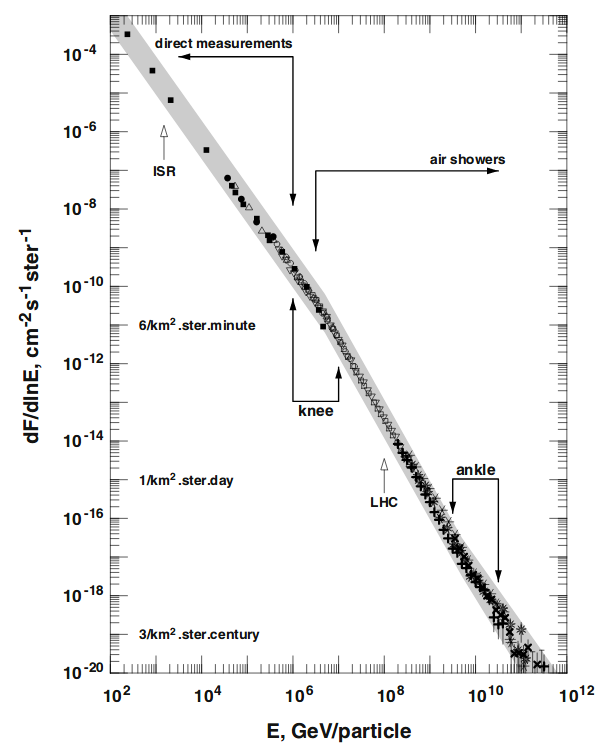
\includegraphics[width=\textwidth]{chapters/pix/CosmicRay_Spectrum.png}
\caption{Measured energy spectrum of cosmic-rays from 100 GeV up to the highest detected energy.}
\label{fig:CR_Spectrum}
\end{figure}

Cosmic-rays have been detected over a large range of energies from GeV (10$^9$ \ eV) to above EeV (10$^18$ \ eV). Spectrum in Figure \ref{fig:CR_Spectrum} shows the break at the knee and ankle and which type of experiments are most suited to measurement each part. Cosmic-ray spectrum starts out at E$^{-2}$ \ and can be as steep as E$^{-2.7}$ at the highest energies.

Cosmic-rays can consist of protons to iron. 

CR spectrum has many feature. Main features are the knee, second knee and ankle. The knee is around 3 $\times$ 10$^{15}$.

Pierre Auger Observatory measurement of isotropy that shows that the cosmic-ray spectrum changes from predominately galactic to extra-galactic at the ankle.

Predicted Greisen-Zatsepin-Kuz’min (GZK) cut-off about 6 $\times$ 10$^{19}$. Cosmic-rays above this energy are theorised to interact with the cosmic microwave background radiation. Greisen independently of Kuz'man and Zatsepin all predicted this energy loss.

Pierre Auger Observatory measurement of Xmax and the second moment $\sigma$(Xmax) has mass composition information as well how this changes as a function of energy.

Mechanisms involved must be able to accelerate cosmic-ray particles to energies exceeding 10$^{20}$ eV. The acceleration region must have the size of the order of the Larmor radius ($r_L$) to be capable of producing a particle of this energy. The Larmor radius is calculated
\begin{equation}
r_L = \frac{p_{\perp}}{Z q_e B}
\end{equation} 
where $Z$ is the atomic number of the particle, $p_{\perp}$ is the momentum perpendicular to the magnetic field, $B$ is the magnetic field strength and $q_e$ is the charge of an electron. There are two possible categories of acceleration: Bottom-Up processes and Top-Down processes.

Bottom-Up processes are where low energy particles are accelerated up to higher energy particles. Proposed bottom-up scenarios include stochastic acceleration. Stochastic acceleration of charged particles was first suggested by Enrico Fermi in 1949. It involves the repeated interaction of charged cosmic-rays with moving clouds of magnetised plasma in the interstellar medium. Magnetised clouds move with random velocities and charged cosmic-rays have a chance of either gaining or losing energy during an interaction. This process can explain the observed power law energy spectrum of cosmic-rays.

Top-Down processes are proposed mechanisms where ultra  high energy cosmic-rays do not obtain their energy from an acceleration process. Their energy is imparted to these particles via the decay of supermassive ($m_X > 10^{20}$ GeV) relic particles from the Big Bang. These relic particles are known generically as `X' particles. X particles decay into quarks and leptons. The quarks can then form jets of pions, with a small proton component. The top-down mechanisms are able to produce ultra high energy cosmic-rays with energies up to ~ m$_X$, however they also predict the production of copious quantities of high energy photons and neutrinos.

Cosmic-rays lose energy as they travel throughout the universe. For protons the main energy loss is through photoproduction on astrophysical photon fields. For cosmic-rays with energies around 10$^{20}$ eV, they can interact with any photon field. The most common and better known photon field is the Cosmic Microwave Background radiation. For nuclei, photo-disintegration can also occur, which results in the ejection of one or more nucleons from the nucleus.

\section{Production Method and Sources}

- Bottom-Up Acceleration 

Supernova explosions 

AGN jets

other energetic processes

dark matter annihilations.

- Top-Down Acceleration

Decay of massive relic particles

Typically associated with new physics beyond the standard model